%
% $RCSfile: extreme_programming.tex,v $
%
% Copyright (C) 2002-2008. Christian Heller.
%
% Permission is granted to copy, distribute and/or modify this document
% under the terms of the GNU Free Documentation License, Version 1.1 or
% any later version published by the Free Software Foundation; with no
% Invariant Sections, with no Front-Cover Texts and with no Back-Cover
% Texts. A copy of the license is included in the section entitled
% "GNU Free Documentation License".
%
% http://www.cybop.net
% - Cybernetics Oriented Programming -
%
% http://www.resmedicinae.org
% - Information in Medicine -
%
% Version: $Revision: 1.1 $ $Date: 2008-08-19 20:41:06 $ $Author: christian $
% Authors: Christian Heller <christian.heller@tuxtax.de>
%

\section{Extreme Programming}
\label{extreme_programming_heading}
\index{Extreme Programming}
\index{XP}
\index{Iterative Structure}
\index{Iteration in XP}
\index{Development in XP}
\index{Collective Code Ownership in XP}
\index{User Stories}
\index{Release Planning}
\index{Learn and Communicate}
\index{Stand Up Meeting}
\index{Free and Open Source Software}
\index{FOSS}
\index{The Cathedral and the Bazar}

\emph{Extreme Programming} (XP) uses the idea of an iterative structure as
explained in section \ref{iterative_process_heading}, with the difference that
it contains not only one but many cycles to assure sufficient feedback. The whole
process can be cascaded and split into more fine-grained processes, for example
\emph{Iteration}, \emph{Development} and \emph{Collective Code Ownership}.
Figure \ref{xp_figure} shows a strongly simplified view of the XP methodology,
with emphasis on its nested structure and multiple iterations. Better and more
detailed overviews are given in \cite{xp}.

\begin{figure}[ht]
    \begin{center}
        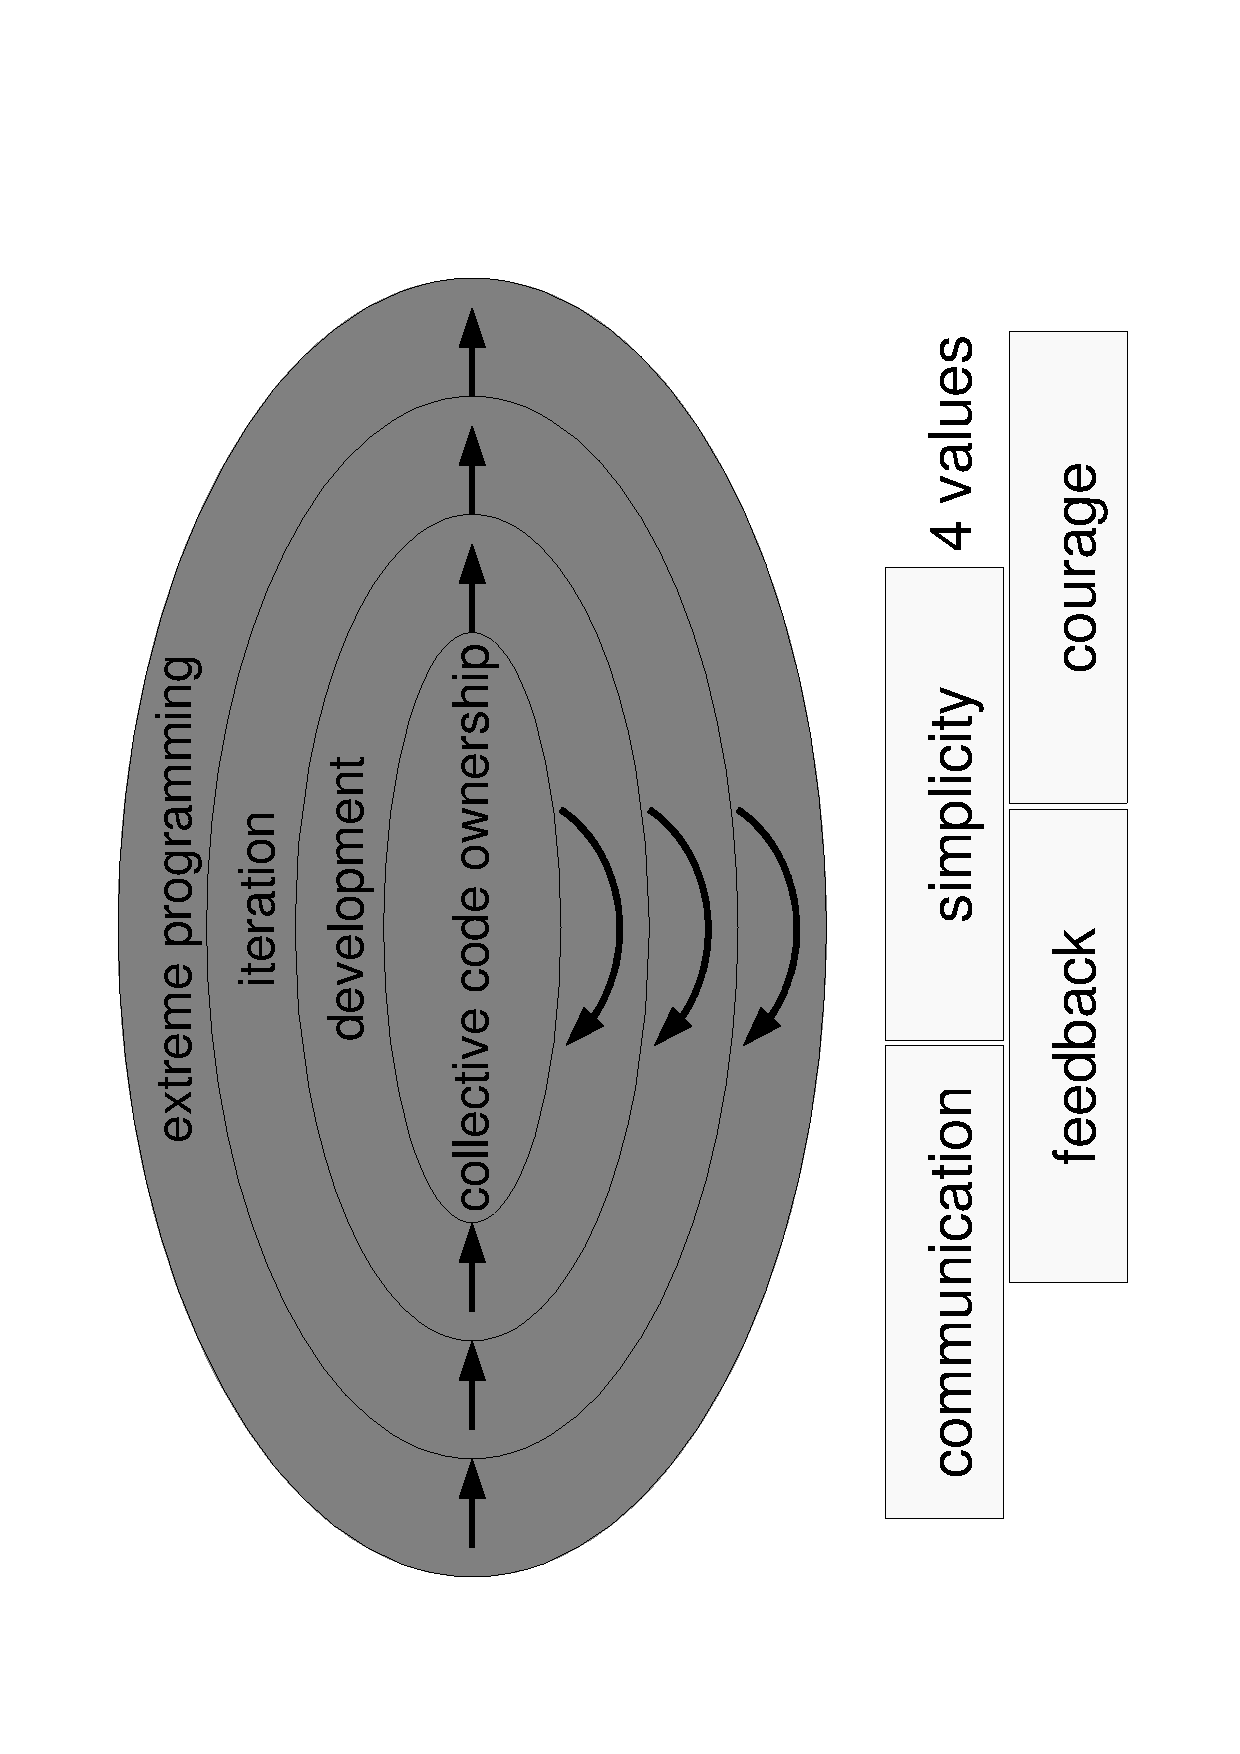
\includegraphics[scale=0.3,angle=-90]{graphic/xp.pdf}
        \caption{Extreme Programming (strongly simplified)}
        \label{xp_figure}
    \end{center}
\end{figure}

In some way or the other, the classical process phases as first mentioned in
section \ref{waterfall_process_heading} also appear in XP, although they may
have different names or a modified meaning. The requirements document, for
example, is replaced by so-called \emph{User Stories}, which are similar to
usage scenarios (except that they are not limited to describing a user
interface), but not to be mixed up with use cases \cite{xp}. Also, a number of
new phases like \emph{Release Planning} appear and more fine-granular
activities like \emph{Learn and Communicate} or \emph{Stand Up Meeting} are
added. The basis and starting point of each XP project are four common values:

\begin{itemize}
    \item[-] Communication
    \item[-] Feedback
    \item[-] Simplicity
    \item[-] Courage
\end{itemize}

The last decade has shown several pushes and increasingly greater support for
\emph{Free and Open Source Software} (FOSS) \cite{opensource}. What makes this
software so successful, besides the fact that its source code is open and
freely available, is its astonishingly fast development model. Well, there
surely are as many different development methodologies as there are FOSS
projects out there, but many of them would probably, at least partly,
match into XP. Additionally, however, there are a few significant differences
that characterise \emph{Open Source Development}. Among them are
\cite{fowlernewmethodology}:

\begin{itemize}
    \item[-] Collaboration between physically distributed teams
    \item[-] Maintainer responsible for overall coordination and design
    \item[-] Highly parallelisable debugging
\end{itemize}

In his book \emph{The Cathedral and the Bazar} \cite{raymond}, Eric S. Raymond
provides further insights. Popular slogans taken from it are: \textit{Release
early and often!}, \textit{Delegate everything you can!} or: \textit{Be open to
the point of promiscuity!} He recommends to foster a community of developers,
lead by \emph{Doing} and \emph{Good Humour}. Yet Tim Churches reminds people not
to take Raymond's recommendations as dogma \cite{openhealth}:

\begin{quote}
    Although Eric S. Raymond's \ldots\ essay brought one particular FOSS
    development paradigm to a lot of people's attention, it may have also done
    the FOSS movement a disservice by making people think that the 'bazaar'
    approach is the only way in which FOSS can be developed.
\end{quote}

Instead, each project should pick a methodology that best suits its needs, may
it be cathedral- or bazaar-like.
